In the following subsections the performance of the different algorithms is tested for different kinds of inputs.
The exact distributions of the input are explained separately in each subsection.
The procedure for each comparison is always the same. A random input is generated according to the distribution and then solved by every algorithm.
All algorithms had the same two stopping conditions.
The first was reaching a perfect partition and the second was taking more than $100 \cdot n\ln(n)$ steps.
If either of these condition was met, the algorithm returned the current best solution.
This step is repeated 1000 times.
The results are presented in a table containing multiple statistics for each algorithm over all 1000 runs.

\begin{tabular}{c|c}
      column name     & meaning                                                         \\ \hline
      algo type       & type of algorithm (RLS, RLS-N, RLS-R, (1+1)EA or pmut)          \\
      algo param      & parameter of the algorithm or '-' if it is the standard variant \\
      avg mut/change  & average \#bits flipped for iterations leading to an improvement \\
      avg mut/step    & average \#bits flipped for any iteration                        \\ \hline
      total avg count & average \#iterations for all runs                               \\
      avg eval count  & average \#iterations of runs returning an optimal solution      \\
      max eval count  & maximum \#iterations of runs returning an optimal solution      \\
      min eval count  & minimum \#iterations of all runs                                \\ \hline
      fails           & number of runs that did not find an optimal solution            \\
      fail ratio      & ratio of unsuccessful runs to all runs                          \\
      avg fail dif    & average value of $b_F-b_E$ for non-optimal solutions            \\
\end{tabular}

Firstly the different variants of the RLS are compared with values of $k \in\{2,3,4\}$, then the performance of the (1+1) EA with static mutation rate $c/n$ with $c \in{1,2,3,5,10,50,100}$ and lastly the performance of the $pmut_\beta$ mutation operator with the parameter $\beta \in \{-1.25, -1.5, \dots, -2.75,-3.0,-3.25\}$. Additionally the best variants of each algorithm are compared in another 1000 runs.

The first analysed inputs are inputs following a binomial distribution \textasciitilde$B(m,p)$ as those inputs have been researched in the previous subsection.
The results showed that the expected value of a single number is the main driver for the amount of perfect partitions the input has.
The results also suggested the inputs tend to have more perfect partitions if the expected value is lower.
The more perfect partitioned an input has relative to the number of all possible partitions, the more likely the different RSHs are to find one of those.
Therefore researching inputs with higher expected values seems more interesting but generating higher values takes more time with a random number generator that needs $\mathcal{O}(mp)$ time.
To keep the time for generating one set of numbers reasonable the values chosen for all tests are $m=10000, p=0.1, n=10000$ with the expected value for a single number being $mp=1000$.
Figure~\ref{fig:binDistExample} shows a random binomial distributed input of length $n=10000$.
All elements are sharply concentrated around the expected value with all values being at $1000\pm200$.
So after the reaching a difference between the two bins of below $(1000-200)/2=400$ the algorithm can no longer achieve an improvement by flipping a single bit.

\begin{figure}[h]
      \caption{Distribution of a random binomial input}
      \centering
      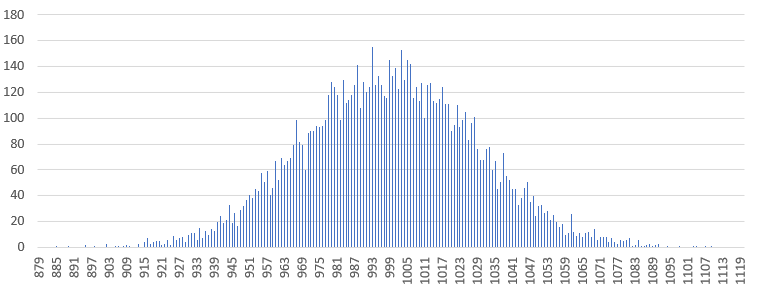
\includegraphics[width=0.7\textwidth]{figures/images/numberGenerator/binomialDistributionForN10000p0_1.png}\label{fig:binDistExample}
\end{figure}